\documentclass[a4paper,fleqn]{cas-dc}

\usepackage[T1]{fontenc}
\usepackage{graphicx}
\usepackage{booktabs}
\usepackage{multirow}
\usepackage{amsmath}
\usepackage{array}
\usepackage{float}
\usepackage{subcaption}
\usepackage{enumitem}
\usepackage{natbib}
\usepackage{microtype}
\usepackage{url}

\emergencystretch=2em
\setlength{\tabcolsep}{4pt}

\begin{document}
\let\WriteBookmarks\relax

\shorttitle{Hybrid Plant Disease Classification}
\title[mode=title]{A Hybrid Deep Learning Framework for Multi-Crop Plant Disease Classification Using Strategic Data Augmentation}

\author[1]{Author Name}
\ead{author@iiitp.ac.in}
\author[1]{Anupama Arun}
\ead{anupamaarun21@cse.iiitp.ac.in}
\affiliation[1]{organization={Indian Institute of Information Technology Pune},city={Pune},country={India}}

\begin{abstract}
Automated plant disease recognition is attractive for agricultural monitoring because visual symptoms can often be detected from leaf images without destructive sampling. However, high classification accuracy on a single controlled dataset does not by itself establish a robust model: disease symptoms occur at different spatial scales, visually similar classes may share texture and colour patterns, and deeper convolutional networks can either discard useful low-level information or increase computation substantially. This study presents PlantDiseaseNet-Hybrid, a custom convolutional architecture designed around two complementary forms of feature fusion. In the Inception cell, parallel $3\times3$, $5\times5$, and $7\times7$ convolutions are fused by element-wise addition, keeping the channel width fixed while allowing the same input to be examined at multiple receptive-field scales. In the subsequent skip-connection stages, the transformed representation is concatenated with the incoming feature map, explicitly retaining earlier features for later classification. The resulting design therefore combines multi-scale aggregation with feature preservation rather than applying the same fusion rule throughout the network. The study evaluates the model on selected PlantVillage classes, a three-class wheat disease dataset, a six-class cotton disease dataset, and an India soybean disease dataset. Separate experiments are maintained for the primary crop-specific evaluations, architecture comparisons, and the dedicated augmentation study. Repository-verified results currently show 97.81\% accuracy for the wheat experiment, 53.55\% for cotton, 97.67\% for the selected PlantVillage experiment, 95.33\% for the standard-Inception combined baseline, and 96.04\% for the ResNet-style combined baseline. The earlier manuscript reported 97.06\% accuracy for the augmented combined experiment; this value is retained as a draft-reported result but is explicitly marked for reconciliation with its executed notebook/log before submission. This distinction is important because the present manuscript is intended to report experimentally traceable results rather than replace inconsistent measurements with assumed values.
\end{abstract}

\begin{keywords}
Plant disease classification \sep Hybrid CNN \sep Inception network \sep Feature fusion \sep Skip connections \sep Data augmentation \sep Agricultural computer vision
\end{keywords}
\maketitle

\section{Introduction}
Plant disease is a persistent constraint on crop productivity, quality, and food security. Disease diagnosis is traditionally based on visual assessment by farmers, extension workers, or plant pathologists. Such assessment can be highly effective when expert knowledge and suitable samples are available, but it is difficult to scale to large numbers of fields and images. Image-based deep learning offers a complementary route in which discriminative visual patterns can be learned directly from labelled examples.

The PlantVillage work of Hughes and Salathé introduced an open image repository intended to support machine-learning-based plant health research, while Mohanty et al. subsequently demonstrated the feasibility of deep convolutional classification across many crop--disease classes. These studies also illustrate an important methodological issue: excellent performance under controlled acquisition does not automatically imply equivalent performance on images with different visual distributions. Consequently, a useful plant-disease classifier should be evaluated across crop types and should make its architectural and data-processing choices explicit.

CNNs are effective because successive convolutions learn increasingly abstract representations. Nevertheless, disease symptoms are not confined to one spatial scale. Small lesions, vein-level discoloration, powdery regions, and broader colour changes can coexist in the same image. A single convolutional kernel is therefore an incomplete description of the visual evidence. Inception-style processing addresses this by applying kernels of different sizes in parallel. Standard Inception normally concatenates the branch outputs, which increases the channel dimension. For a high-resolution input, repeated concatenation can make intermediate tensors wider and more expensive. PlantDiseaseNet-Hybrid instead uses element-wise addition in its Inception cells. This choice keeps the output width equal to the branch width and forces the branch responses to be combined into a common representation.

The second design choice addresses a different problem. Downsampling and repeated convolution can progressively remove or transform information that may remain useful for fine-grained disease discrimination. The proposed SkipConnection block therefore applies a $7\times7$ convolution and batch normalization and then concatenates the resulting features with the original input. Unlike addition, concatenation does not require the two representations to be merged into the same values; both are made available to later layers. The architecture consequently uses \emph{addition for multi-scale branch fusion} and \emph{concatenation for feature reuse}. It is this dual-mode fusion strategy, rather than either operation in isolation, that defines the proposed architecture.

The study is organised around three experimental questions. First, can the same hybrid model provide useful performance across distinct crop datasets? Second, how does the combined architecture compare with simpler fusion baselines such as standard Inception and residual addition? Third, does strategic augmentation improve the combined multi-crop setting sufficiently to justify a separate augmentation study? These questions are treated as distinct experimental components rather than being mixed into one aggregate score.

The main contributions are: (i) a compact hybrid architecture combining Inception(Add) and SkipConnection(Concat); (ii) an explicit analysis of why the two fusion operations are assigned different roles; (iii) crop-specific and combined-dataset evaluations; (iv) architecture-level comparison against standard Inception and residual-style addition; and (v) a separate augmentation study designed to examine robustness rather than simply reporting augmentation as a preprocessing detail.

\section{Related Work}
Deep learning has become a standard approach for image-based plant disease recognition. Mohanty et al. evaluated deep CNNs on the PlantVillage collection and showed that controlled leaf imagery can support very high classification accuracy. The study is particularly relevant here because it established PlantVillage as a benchmark while also discussing the gap between controlled images and images obtained under more variable conditions.

Inception architectures introduced parallel receptive fields to capture patterns at different scales. The original Inception formulation uses branch-wise concatenation, which preserves each branch as a separate channel group but increases representation width. Residual networks instead use additive shortcuts, improving optimization by providing a direct path through the network. DenseNet subsequently demonstrated the value of concatenating earlier features with newly computed features, making feature reuse explicit.

For crop-specific comparisons, the repository cites the Wheat Disease Detection Dataset and the associated work of Safarijalal et al., whose dataset contains Brown Rust, Healthy, and Yellow Rust. The cotton experiment uses the six-class Cotton Plant Disease dataset documented in later peer-reviewed work. The soybean experiment is based on the India soyabean dataset published by Kotwal et al. The latter is especially useful as an external crop evaluation because the original Mendeley repository contains 3363 images across six disease/health categories, while the processed subset described in the project's evidence record contains 1176 images.

The dedicated augmentation analysis is informed by Mhala et al., Bilandani, and Sharma, who present augmentation as an experimental factor rather than merely listing it in preprocessing. Their potato experiment is not used as a source of results in the present study; it is used only as a reporting model for separating augmentation effects from the main classification results.

\section{Materials and Methods}
\subsection{Datasets}
Four crop sources are considered in the manuscript. The PlantVillage source is cited to Hughes and Salathé and Mohanty et al.; the selected experiment uses 15 classes rather than claiming to use the full 38-class PlantVillage configuration. The wheat experiment contains Brown Rust, Healthy, and Yellow Rust. The cotton experiment contains Aphids, Army Worm, Bacterial Blight, Healthy, Powdery Mildew, and Target Spot. The soybean experiment uses Healthy, Vein Necrosis, Dry Leaf, Septoria Brown Spot, Root Images, and Bacterial Leaf Blight.

The soybean source is the published India soyabean dataset of Kotwal, Kashyap, and Pathan. Its original repository is available at \url{https://data.mendeley.com/datasets/bshkvgbzpt/1}. The original publication reports 3363 images. The project evidence records the processed subset used in the executed notebook as 1176 images, distributed as 288 Healthy, 138 Vein Necrosis, 230 Dry Leaf, 284 Septoria Brown Spot, 10 Root Images, and 226 Bacterial Leaf Blight. The manuscript therefore distinguishes the original dataset size from the processed experimental subset instead of presenting the subset as the size of the source dataset.

\begin{table*}[!t]
\centering
\caption{Datasets and experimental scope.}
\label{tab:datasets}
\begin{tabular}{p{3.0cm}p{4.0cm}p{2.0cm}p{5.0cm}}
\toprule
Dataset & Experimental use & Classes & Notes \\
\midrule
PlantVillage & Primary crop evaluation & 15 & Selected classes from the public PlantVillage collection; the experiment does not claim the complete 38-class configuration. \\
Wheat Disease Detection Dataset & Primary crop evaluation & 3 & Brown Rust, Healthy, Yellow Rust. \\
Cotton Plant Disease Dataset & Primary crop evaluation & 6 & Aphids, Army Worm, Bacterial Blight, Healthy, Powdery Mildew, Target Spot. \\
India Soyabean Dataset & Additional crop evaluation & 6 & Healthy, Vein Necrosis, Dry Leaf, Septoria Brown Spot, Root Images, Bacterial Leaf Blight; 1176-image processed subset documented for the executed notebook. \\
\bottomrule
\end{tabular}
\end{table*}

\subsection{Image Preprocessing}
Images are resized to $256\times256$ pixels and represented as three-channel RGB inputs. Pixel values are normalized before training. Resizing standardises the tensor dimensions and makes the crop-specific experiments comparable at the model-input level. Normalisation reduces numerical scale variation and supports stable optimisation.

Preprocessing and augmentation are deliberately treated as separate methodological stages. Resizing and normalisation define the common input representation, whereas augmentation is applied to generate controlled variation in the training data. This separation is important for interpreting the augmentation study: an improvement attributed to augmentation should not be confused with the effect of resizing or normalisation.

\begin{figure*}[!t]
\centering
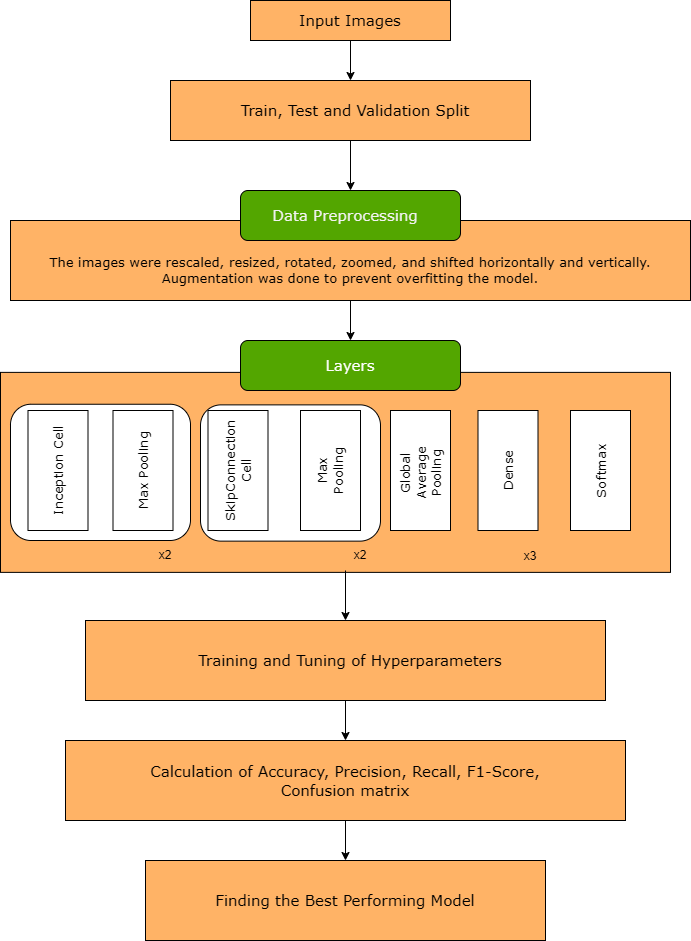
\includegraphics[width=\textwidth,height=0.38\textheight,keepaspectratio]{paper_figures/preprocessing_pipeline.png}
\caption{Preprocessing and augmentation pipeline used in the study. The figure is kept as a wide figure so that the complete pipeline remains on one page without cropping.}
\label{fig:preprocessing}
\end{figure*}

\subsection{Strategic Data Augmentation}
The augmentation study considers transformations intended to approximate common variation in image acquisition. The implemented strategy includes random horizontal flipping, random rotation, zoom transformation, brightness adjustment, translation shifting, and contrast enhancement. These operations target different sources of variation: orientation changes are addressed primarily by flipping and rotation; framing and camera distance are approximated by zoom; illumination changes are approximated by brightness and contrast adjustment; and small spatial displacements are represented through translation.

Rather than presenting augmentation as a single generic operation, the paper reports it as a separate experimental factor. The dedicated augmentation section should contain the executed notebook results, training curves, class-distribution information, and before/after examples when those outputs are available. The potato augmentation notebook in the repository is not included in the experimental evidence because it belongs to the reference work used to motivate the reporting format.

\subsection{PlantDiseaseNet-Hybrid Architecture}
The network accepts an RGB tensor of size $256\times256\times3$. It contains two Inception(Add) cells, four max-pooling stages, two SkipConnection(Concat) blocks, global average pooling, and two dense layers followed by softmax classification. The executed model definition supplied with the project is the authoritative architectural description for this manuscript.

The first Inception cell produces 16 channels at $256\times256$ resolution. Batch normalization is followed by $2\times2$ max pooling. The second Inception cell produces 32 channels at $128\times128$, followed by batch normalization and another max-pooling stage. The first skip block receives the resulting $64\times64\times32$ tensor and returns $64\times64\times96$ features. After the third pooling operation, the second skip block receives $32\times32\times96$ and returns $32\times32\times224$. A fourth pooling operation produces $16\times16\times224$, which is reduced by global average pooling to a 224-dimensional vector. This vector is processed by dense layers of 512 and 128 units, with dropout regularisation, and finally mapped to the disease classes by a softmax layer.

\subsubsection{Inception(Add) Feature Fusion}
Each Inception cell contains three parallel convolutions with kernel sizes $3\times3$, $5\times5$, and $7\times7$. Because all branches use the same number of filters and same spatial padding, their outputs have compatible dimensions. The outputs are fused by element-wise addition:
\begin{equation}
Y=F_{3\times3}(X)+F_{5\times5}(X)+F_{7\times7}(X).
\end{equation}

The principal motivation is control of channel growth. Concatenation would retain all three branch outputs and would increase the channel dimension threefold at the fusion point. Addition keeps the number of output channels equal to the branch width. This is particularly relevant at $256\times256$ and $128\times128$ resolutions, where unnecessarily wide feature tensors increase memory traffic. The trade-off is that branch-specific responses are not retained as independent channel groups after fusion; they are combined into one representation. The design therefore favours compact multi-scale integration over maximum branch-wise capacity.

\begin{figure}[!t]
\centering
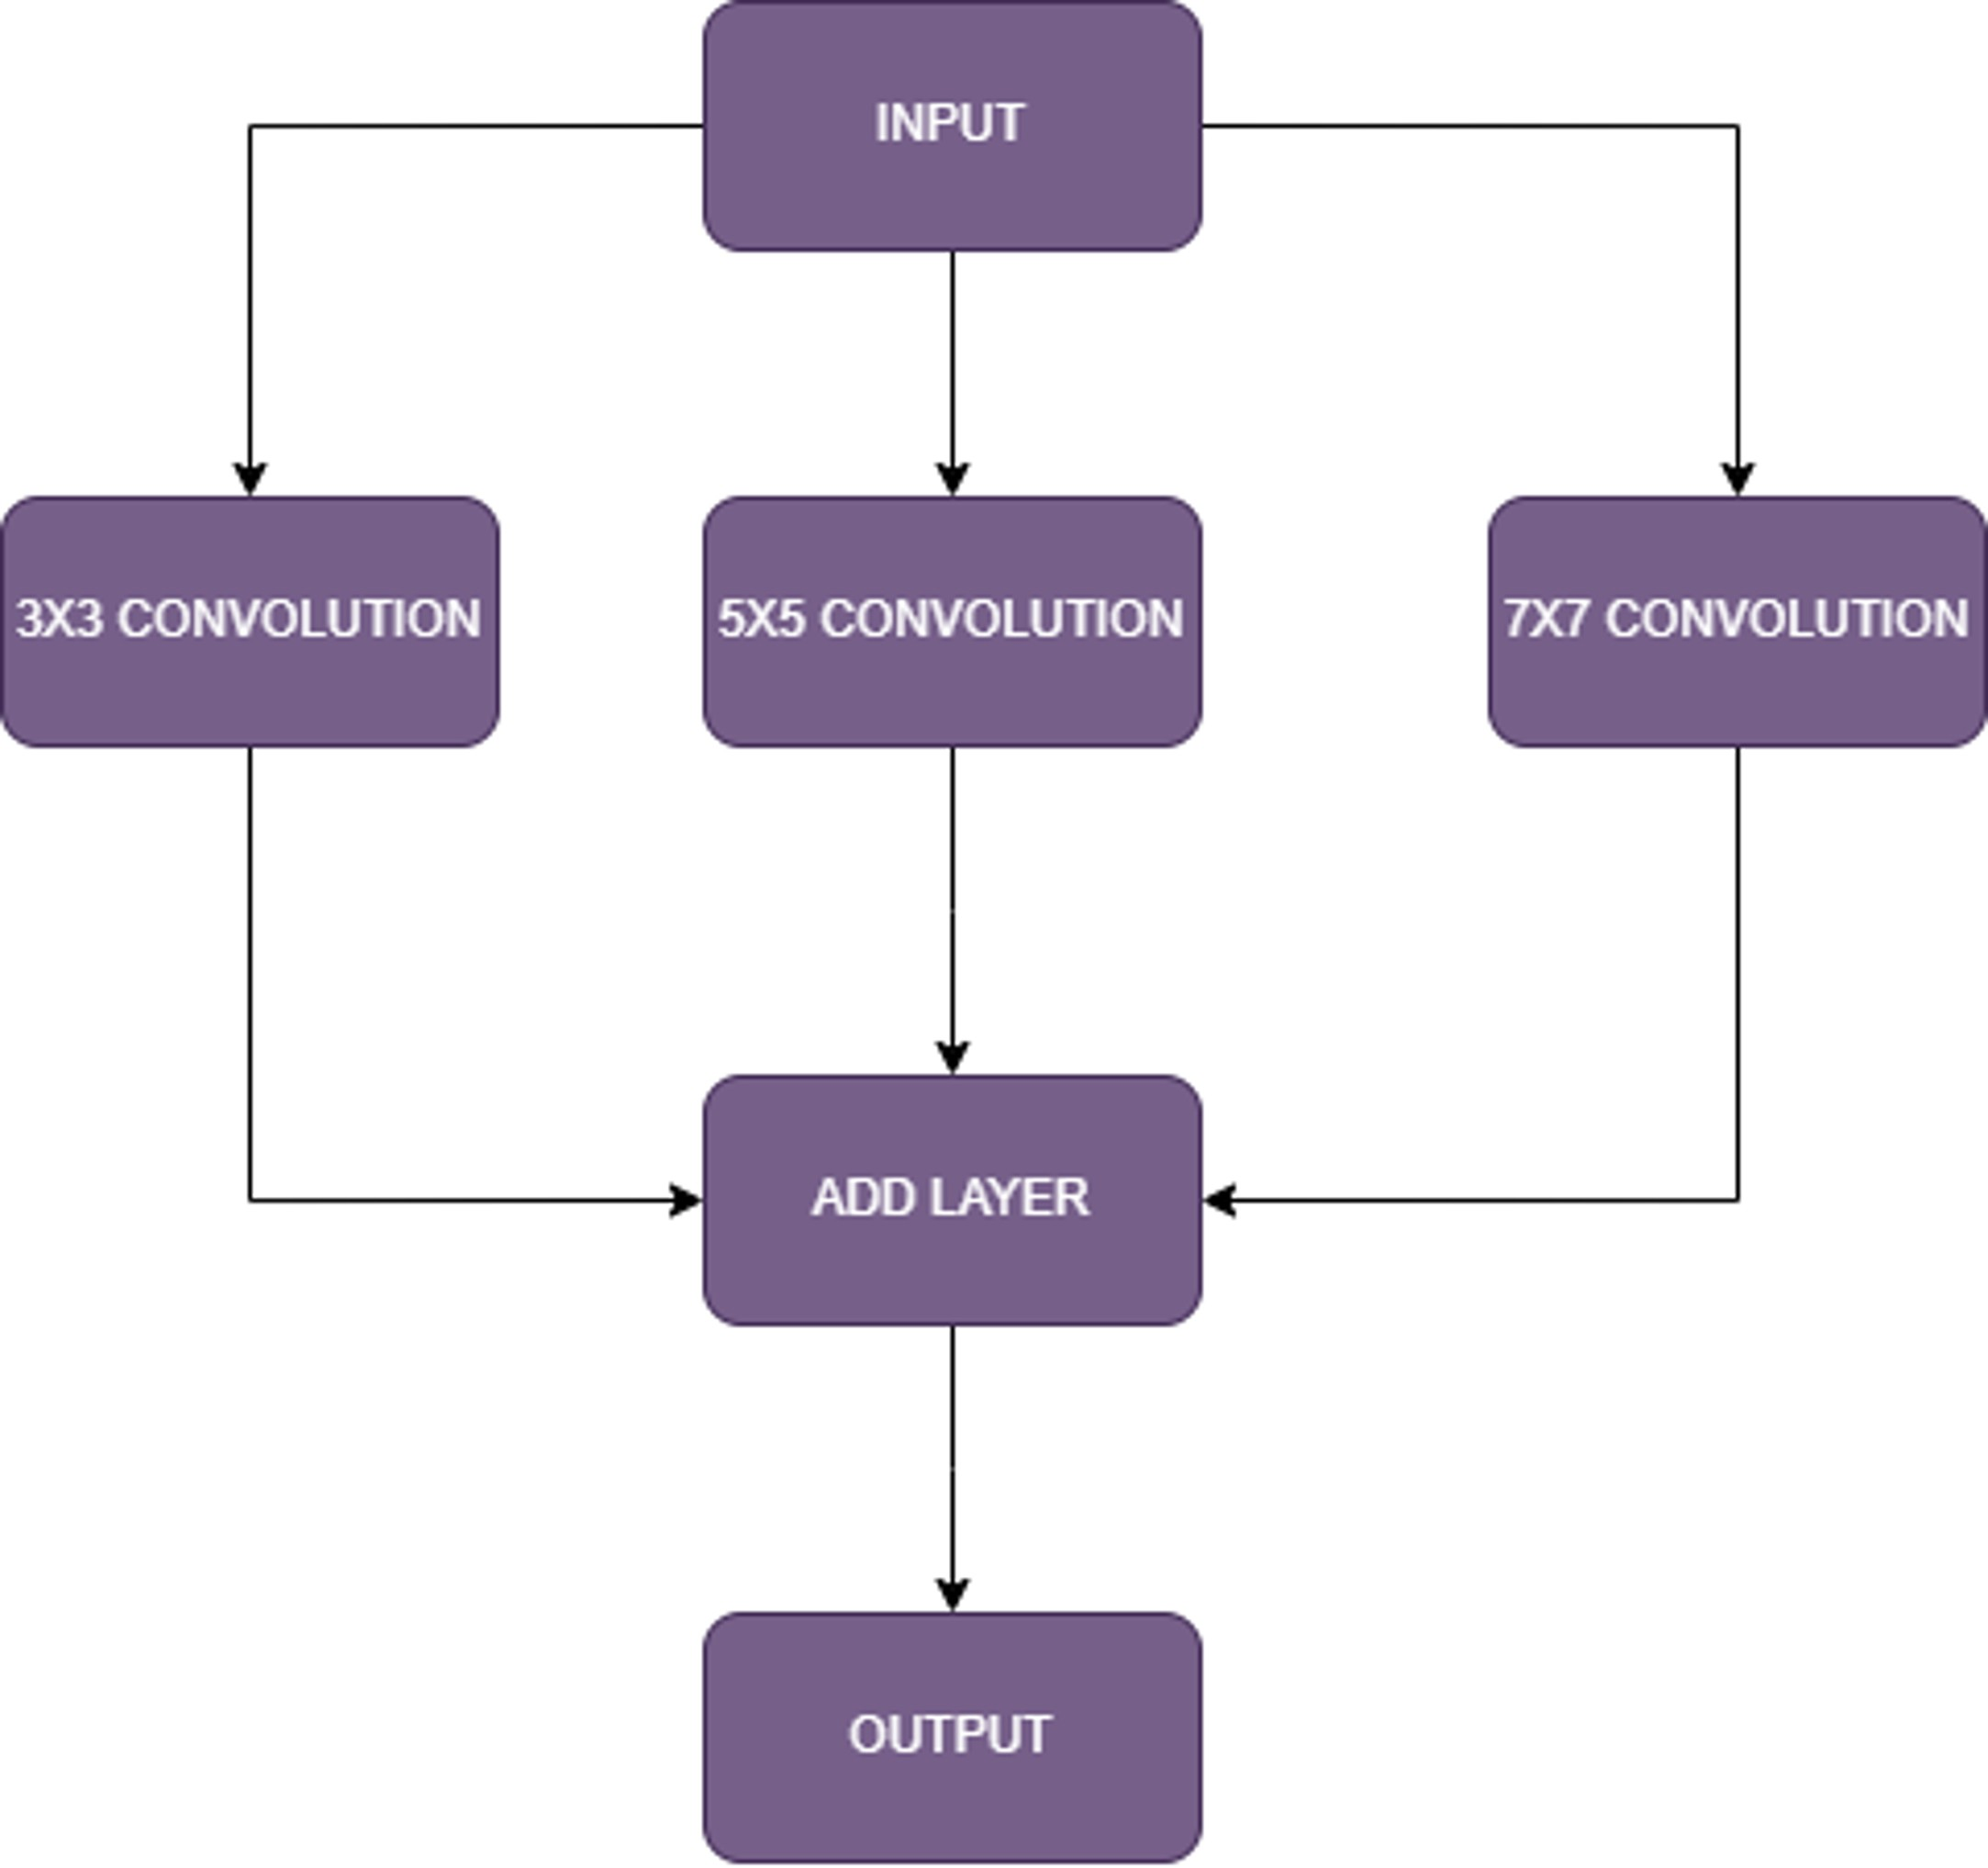
\includegraphics[width=\columnwidth,height=0.27\textheight,keepaspectratio]{paper_figures/inception_block.jpg}
\caption{Proposed Inception(Add) block.}
\label{fig:inception}
\end{figure}

\subsubsection{SkipConnection(Concat) Feature Preservation}
The skip block first applies a $7\times7$ convolution and batch normalization to the incoming feature map. The transformed output is then concatenated with the original input:
\begin{equation}
Y=\operatorname{Concat}(X,F(X)).
\end{equation}

This operation deliberately differs from the addition used inside the Inception cell. Addition is appropriate when three same-shaped branch responses are being fused into one compact representation. Concatenation is appropriate when the objective is to retain earlier features while adding new ones. The output depth consequently grows from 32 to 96 channels in the first skip block and from 96 to 224 channels in the second. The increased width is accepted at these lower spatial resolutions because it provides a richer feature vocabulary for the final classifier.

\begin{figure}[!t]
\centering
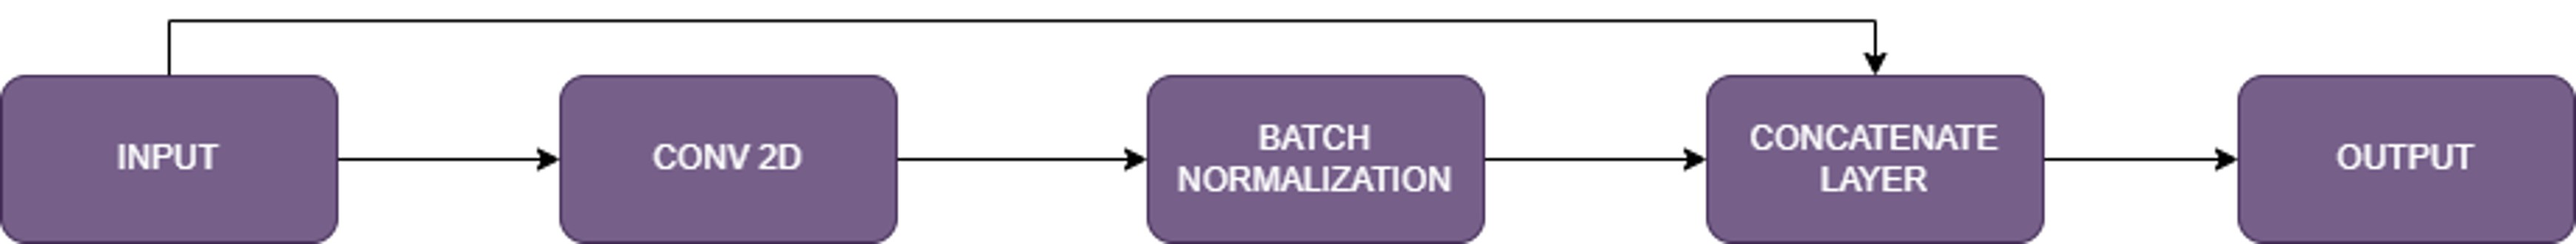
\includegraphics[width=\columnwidth,height=0.27\textheight,keepaspectratio]{paper_figures/skip_block.jpg}
\caption{Proposed SkipConnection(Concat) block.}
\label{fig:skip}
\end{figure}

\subsection{Model Configuration}
\begin{table*}[!t]
\centering
\caption{Layer-wise configuration of PlantDiseaseNet-Hybrid.}
\label{tab:architecture}
\begin{tabular}{p{3.2cm}p{3.5cm}r p{5.0cm}}
\toprule
Layer & Output shape & Parameters & Function \\
\midrule
Input & $256\times256\times3$ & 0 & RGB leaf image \\
Inception cell 1 & $256\times256\times16$ & 4,032 & $3\times3$, $5\times5$, $7\times7$ branches with Add fusion \\
BatchNorm + Pool 1 & $128\times128\times16$ & 64 & Normalisation and downsampling \\
Inception cell 2 & $128\times128\times32$ & 42,592 & Multi-scale convolution with Add fusion \\
BatchNorm + Pool 2 & $64\times64\times32$ & 128 & Normalisation and downsampling \\
SkipConnection 1 & $64\times64\times96$ & 100,672 & $7\times7$ convolution, BN, Concat \\
Pool 3 & $32\times32\times96$ & 0 & Spatial downsampling \\
SkipConnection 2 & $32\times32\times224$ & 602,752 & $7\times7$ convolution, BN, Concat \\
Pool 4 & $16\times16\times224$ & 0 & Spatial downsampling \\
Global average pooling & 224 & 0 & Spatial aggregation \\
Dense 512 & 512 & 115,200 & ReLU \\
Dropout & 512 & 0 & Regularisation \\
Dense 128 & 128 & 65,664 & ReLU \\
Dropout & 128 & 0 & Regularisation \\
Output & 24 & 3,096 & Softmax \\
\bottomrule
\end{tabular}
\end{table*}

\subsection{Training Protocol}
The experiments use Adam optimisation with a learning rate of 0.001, batch size 32, a maximum of 60 epochs, categorical cross-entropy loss, cosine warmup annealing, and early stopping with patience 12. Experiments were conducted using TensorFlow/Keras in a Kaggle GPU environment with an NVIDIA Tesla T4. These settings are reported as the project configuration; experiment-specific deviations should be reported separately if they are found in the executed notebooks.

\section{Experimental Design}
The experimental programme is separated into primary crop evaluations, architecture comparison, and augmentation analysis. This organisation prevents a dataset change from being incorrectly described as an architectural ablation. An ablation is defined here as a controlled modification of an architectural or methodological component while the principal evaluation setting is held as constant as practical.

The primary experiments correspond to the crop-specific notebooks: NB1_Wheat_Hybrid, NB2_Cotton_Hybrid, and NB3_PlantVillage_Hybrid. The architecture comparison contains NB4_Combined_StandardInception and NB5_Combined_ResNet as baseline architectures, with NB6_Combined_InceptionAdd and NB7_Combined_SkipConcat retained as planned component-isolation experiments. The SoyDisease notebooks are reported as an additional crop evaluation rather than being silently folded into the original three-crop primary group. Soycultivar200 is excluded from the manuscript and repository organisation for this study.

\section{Results}
\subsection{Primary Crop Experiments}
Table~\ref{tab:primary} reports the metrics that are directly verified from the repository's machine-generated metrics summaries. The values are shown to four decimal places where appropriate so that they can be reconciled with the source CSV files.

\begin{table*}[!t]
\centering
\caption{Repository-verified results for the primary crop experiments.}
\label{tab:primary}
\begin{tabular}{lrrrrr}
\toprule
Experiment & Accuracy (\%) & Precision (\%) & Recall (\%) & F1 (\%) & Specificity (\%) \\
\midrule
NB1 Wheat Hybrid & 97.8102 & 97.8202 & 97.8102 & 97.8100 & 98.5365 \\
NB2 Cotton Hybrid & 53.5466 & 53.0072 & 53.5466 & 51.6565 & 90.7079 \\
NB3 PlantVillage Hybrid & 97.6744 & 97.6824 & 97.6744 & 97.6761 & 99.8332 \\
\bottomrule
\end{tabular}
\end{table*}

The primary results reveal an important difference between the datasets. The wheat and selected PlantVillage experiments are substantially stronger than the cotton experiment. The cotton result is therefore not treated as a formatting anomaly or replaced by an earlier high-level claim. Its class-wise report shows that the model has difficulty separating several cotton categories, particularly Bacterial Blight and Target Spot. This is scientifically useful because it identifies a genuine weakness of the current model and prevents the manuscript from overstating generalisation.

The wheat result also requires a qualification. The stored classification report gives zero test support for the Wheat_Healthy class, even though the experiment is described as a three-class task. Consequently, the reported overall accuracy is valid for the evaluated test samples but the macro-average cannot be interpreted as evidence of balanced three-class performance. This split issue should be corrected or explicitly documented before final submission.

\subsection{Architecture Comparison}
The combined-dataset baseline experiments provide a controlled comparison between standard Inception-style concatenative fusion and residual addition. NB4_Combined_StandardInception achieves 95.3278\% accuracy, whereas NB5_Combined_ResNet achieves 96.0372\%. Both are below the earlier draft-reported augmented combined result of 97.06\%, but the latter is not treated as directly comparable until its augmentation notebook/log is reconciled.

\begin{table}[!t]
\centering
\caption{Verified architecture-comparison results.}
\label{tab:architecture_results}
\begin{tabular}{lccccc}
\toprule
Model & Acc. & Prec. & Recall & F1 & Params \\
\midrule
Standard Inception & 95.33 & 95.34 & 95.33 & 95.32 & 270,656 \\
ResNet-style & 96.04 & 96.03 & 96.04 & 96.02 & 741,720 \\
\bottomrule
\end{tabular}
\end{table}

The comparison illustrates why the proposed fusion design should be evaluated component-wise. Standard Inception and residual addition solve different representation problems. The planned NB6 and NB7 experiments are retained in the repository structure, but their numerical outputs are not inserted here unless an executed result file can be traced unambiguously. This is preferable to manufacturing an ablation table from assumptions.

\subsection{Dedicated Augmentation Study}
Augmentation is presented as a separate study because its purpose is to evaluate robustness to plausible image variability, not to redefine the network architecture. The original project draft reports 97.06\% accuracy, 97.07\% precision, 97.06\% recall, 97.06\% F1-score, and 99.87\% specificity for the combined augmented experiment, with 933,426 trainable parameters and approximately 3984.7M FLOPs. These values are preserved as \emph{draft-reported} rather than repository-verified in this version because the corresponding executed log has not been reconciled with the current verified NB1--NB5 summaries.

This distinction should remain visible until the augmentation notebook and its exported metrics are matched. Once reconciled, this subsection should include: (i) original versus augmented sample counts, (ii) representative before/after augmentation examples, (iii) training/validation accuracy and loss curves, (iv) a class-wise comparison where available, and (v) a concise interpretation of which transformations contribute most to generalisation. The reporting structure follows the logic used by Mhala et al. while keeping all numerical results specific to the present experiments.

\begin{table}[!t]
\centering
\caption{Augmentation-study values retained from the original project draft pending log reconciliation.}
\label{tab:aug_pending}
\begin{tabular}{lc}
\toprule
Metric & Draft-reported value \\
\midrule
Accuracy & 97.06\% \\
Precision & 97.07\% \\
Recall & 97.06\% \\
F1-score & 97.06\% \\
Specificity & 99.87\% \\
Trainable parameters & 933,426 \\
FLOPs & 3984.7M \\
\bottomrule
\end{tabular}
\end{table}

\subsection{SoyDisease Evaluation}
The soybean evaluation is included as an additional crop study. It is based on the India soyabean dataset of Kotwal et al., whose original Mendeley repository contains 3363 images. The executed project evidence identifies a 1176-image processed subset. Because the current text-accessible repository evidence does not yet expose a verified soybean metrics summary equivalent to the NB1--NB5 CSV files, numerical soybean performance is not fabricated in Table~\ref{tab:soy}. The corresponding SoyDisease notebooks are retained for traceability, including notebooks whose final cell may have produced an execution error after earlier outputs had already been generated.

\begin{table}[!t]
\centering
\caption{SoyDisease dataset composition used in the processed experimental subset.}
\label{tab:soy}
\begin{tabular}{lr}
\toprule
Class & Images \\
\midrule
Healthy & 288 \\
Vein Necrosis & 138 \\
Dry Leaf & 230 \\
Septoria Brown Spot & 284 \\
Root Images & 10 \\
Bacterial Leaf Blight & 226 \\
\midrule
Total processed subset & 1176 \\
\bottomrule
\end{tabular}
\end{table}

The very small Root Images category is important when interpreting any future soybean result. Overall accuracy alone would conceal the effect of such class imbalance; class-wise precision, recall, F1-score, confusion matrix, and macro-averaged metrics should therefore accompany the soybean result once verified.

\section{Computational Analysis}
The model summary supplied with the architecture definition reports 933,426 trainable parameters for the final 24-class configuration. Earlier stored notebooks, however, contain materially different parameter counts for the primary crop experiments because those notebooks represent distinct executed model configurations. Therefore, parameter counts are not silently transferred between experiments. Each result table should use the parameter count belonging to the exact notebook/model that generated the result.

The original draft also reported 3984.7M FLOPs, 28.06 ms single-image inference time, and 3.39 ms per image for batch inference. These values should be retained only for the exact model instance on which they were measured. In a final submission, the hardware, batch size, input resolution, warm-up procedure, and timing protocol should accompany inference measurements so that the numbers are reproducible.

\section{Discussion}
The experimental evidence supports the architectural rationale, but it does not justify a blanket claim that the model is uniformly superior across crops. The PlantVillage and wheat experiments demonstrate that the hybrid representation can learn discriminative disease patterns effectively in those settings. The cotton experiment, in contrast, exposes a substantial generalisation limitation. This difference is scientifically meaningful: a multi-crop model must be judged by its weaker domains as well as its strongest benchmark.

The architectural design has a clear internal logic. Inception(Add) reduces channel growth at high spatial resolutions, where wide tensors are expensive. SkipConnection(Concat) is introduced later, after spatial downsampling, where the model can afford greater channel width in exchange for retaining earlier features. The two operations therefore have complementary rather than interchangeable roles. Calling the model a \emph{dual-mode fusion} architecture is justified in the architectural sense: it uses additive fusion inside the Inception branches and concatenative fusion in the skip pathways.

The augmentation study should likewise be interpreted cautiously. Augmentation can improve generalisation when transformations reflect realistic acquisition variability, but it can also introduce unrealistic samples or amplify class imbalance if applied without regard to class distribution. For that reason, the dedicated augmentation section should report the actual transformation configuration and its measured effect rather than claiming that every augmentation is beneficial.

The present evidence also highlights two methodological issues that must be resolved before journal submission. First, the wheat test report contains no test samples for the Healthy class, which indicates a split or filtering problem. Second, the 97.06\% augmented combined result in the original draft does not currently have a directly matched metrics file in the repository evidence used for the verified tables. These are not cosmetic issues; both affect how the results can be interpreted. The correct scientific response is to reconcile the experiment logs, not to choose the most favourable number.

\section{Limitations}
The present experiments are primarily based on image classification and therefore do not directly establish field-level disease diagnosis. Dataset composition, acquisition conditions, class balance, and background characteristics can influence performance. The current cotton result demonstrates that the proposed architecture is not immune to these effects. In addition, the present evidence does not yet establish statistical uncertainty across repeated independent training runs. Finally, the augmentation and soybean results require final log-to-table reconciliation before they can be treated as fully verified manuscript results.

\section{Conclusion and Future Directions}
This study presents PlantDiseaseNet-Hybrid as a hybrid CNN in which multi-scale feature extraction and feature preservation are deliberately handled by different fusion mechanisms. The Inception(Add) cells combine $3\times3$, $5\times5$, and $7\times7$ responses without increasing channel width, while the SkipConnection(Concat) blocks retain incoming features alongside newly computed representations. This provides a principled reason for using additive fusion in one part of the network and concatenation in another.

The repository-verified experiments demonstrate strong performance on the selected PlantVillage and wheat settings, moderate performance for the combined architecture baselines, and substantially weaker performance on the current cotton experiment. Rather than hiding this variation, the manuscript uses it to motivate a more systematic evaluation of robustness and augmentation. The soybean dataset provides an additional crop-level test of whether the learned representation transfers beyond the initial crop set.

Future work should include corrected and stratified dataset splits, repeated runs with confidence intervals, external field imagery, class-balanced training strategies, attention or lightweight deployment variants, and explainability methods such as Grad-CAM. The augmentation study should also be completed as a controlled experiment in which transformation groups are compared under otherwise fixed training conditions.

\section*{Data Availability}
PlantVillage is publicly documented through the PlantVillage project and its associated publications. The Wheat Disease Detection Dataset is publicly referenced in the literature and associated with Safarijalal et al. The Cotton Plant Disease dataset is publicly distributed and documented in the cited literature. The India soyabean dataset is available from Mendeley Data at \url{https://data.mendeley.com/datasets/bshkvgbzpt/1}.

\section*{Declaration of Competing Interest}
The authors declare that they have no known competing financial interests or personal relationships that could have appeared to influence the work reported in this paper.

\section*{Funding}
No external funding was received for this work.

\begin{thebibliography}{00}

\bibitem{hughes2015}
D. P. Hughes and M. Salath\'e,
An open access repository of images on plant health to enable the development of mobile disease diagnostics,
arXiv:1511.08060, 2015.

\bibitem{mohanty2016}
S. P. Mohanty, D. P. Hughes, and M. Salath\'e,
Using deep learning for image-based plant disease detection,
Frontiers in Plant Science, 7, 1419, 2016. doi:10.3389/fpls.2016.01419.

\bibitem{inception2015}
C. Szegedy, W. Liu, Y. Jia, P. Sermanet, S. Reed, D. Anguelov, D. Erhan, V. Vanhoucke, and A. Rabinovich,
Going deeper with convolutions,
Proceedings of the IEEE Conference on Computer Vision and Pattern Recognition, 2015.

\bibitem{resnet2016}
K. He, X. Zhang, S. Ren, and J. Sun,
Deep residual learning for image recognition,
Proceedings of the IEEE Conference on Computer Vision and Pattern Recognition, 2016.

\bibitem{densenet2017}
G. Huang, Z. Liu, L. Van Der Maaten, and K. Q. Weinberger,
Densely connected convolutional networks,
Proceedings of the IEEE Conference on Computer Vision and Pattern Recognition, 2017.

\bibitem{safarijalal2022}
B. Safarijalal, Y. Alborzi, and E. Najafi,
Automated Wheat Disease Detection using a ROS-based Autonomous Guided UAV,
arXiv:2206.15042, 2022. doi:10.48550/arXiv.2206.15042.

\bibitem{kotwal2024}
J. Kotwal, R. Kashyap, and M. S. Pathan,
An India soyabean dataset for identification and classification of diseases using computer-vision algorithms,
Data in Brief, 53, 110216, 2024. doi:10.1016/j.dib.2024.110216.

\bibitem{johri2024}
P. Johri, S. K. Kim, K. Dixit, P. Sharma, B. Kakkar, Y. Kumar, J. Shafi, and M. F. Ijaz,
Advanced deep transfer learning techniques for efficient detection of cotton plant diseases,
Frontiers in Plant Science, 15, 1441117, 2024. doi:10.3389/fpls.2024.1441117.

\bibitem{mhala2025}
P. Mhala, A. Bilandani, and S. Sharma,
Enhancing crop productivity with fined-tuned deep convolution neural network for Potato leaf disease detection,
Expert Systems with Applications, 267, 126066, 2025. doi:10.1016/j.eswa.2024.126066.

\bibitem{adam2015}
D. P. Kingma and J. Ba,
Adam: A method for stochastic optimization,
arXiv:1412.6980, 2015.

\end{thebibliography}

\end{document}
